


\section{Relevant Text Detection}
\label{cp4:corpus-relevant-text}






Next, we need to determine which 
of the text in the gathered artifacts could provide information that assists a developer in solving her task.
In our corpus, this text represents \textit{golden data} that one can use to design and evaluate automatic tools that assist developers in the identification of information useful to their tasks. 
To produce it, we 
ask experienced developers to
mark the text that they deem useful and that provide information for tasks assigned to them~\cite{nadi2020, Robillard2015, marques2020}.



\subsection{Annotation process}


Our intention is that golden data reflect text that instructs developers to perform important actions to accomplish their task~\cite{Robillard2015, Lotufo2012}.
To this end, we describe the annotators' background, annotation procedures, and the 
the text inspected by the annotators.
% FIXME: find a way to format the standard deviation acronym
\textcolor{white}{\acs{stdv}} % force acronym to appear in the glossary for the time being





\subsubsection{Annotators}


We recruited 3 graduate students with professional programming experience to produce \textit{golden} data for our corpus. Annotators had to have experience with Java development and they also had to be familiar with the types of artifacts they would encounter throughout the annotation process. 
On average, annotators self-reported 3.0 years of professional
programming experience ({\small $\pm$} 1.63, ranging from 1 to 5 years).



\subsubsection{Annotation procedures}



The annotation process started with two tasks, other than the ones in our dataset, so that annotators could familiarize themselves with annotation procedures.
We discussed results from these two tasks with all annotators to ensure consistency over responses to any of the questions annotators had. No changes arose from the two introductory tasks.
After this step, we presented the  tasks in the \acs{DS-android} corpus to the annotators, dividing them into batches of 10 tasks each. 



For each task, including the introductory tasks, annotators had the task description and links to artifacts pertinent to the task at their disposal. We asked annotators to write a short solution plan (250 words maximum~\cite{Rastkar2010}) with instructions that a developer could follow to complete the task successfully. 
The purpose of the plan was to ensure that annotators built enough context about the task.
While perusing artifacts, annotators also had to manually highlight sentences that they deemed useful and that provided information that assisted task completion---instructions similar to the ones used for the creation of the data in Nadi and Treude's study~\cite{nadi2020}
or in the \acs{DS-synthetic} corpus created in Chapter~\ref{ch:characterizing}.


Annotation was facilitated by a tool we created for this purpose. 
Figure~\ref{fig:corpus-annotation-tool} shows a screenshot from the tool in 
action, which works as a browser plug-in. The top-right corner panel in the figure shows the browser extension. When an annotator clicked the \texttt{highlight} button, 
the tool instrumented the HTML of a page identifying individual sentences. The tool then allowed annotators to hover over identified sentences and to select them as relevant by clicking on the hovered text. For example, in the first paragraph, an annotator selected  the sentence
``\textit{In Android 9.0 or higher, you can start another app's activity in lock task mode.}'' as relevant to the Android lock task (Figure~\ref{fig:lock-screen-task}).







\begin{figure}
    \centering
    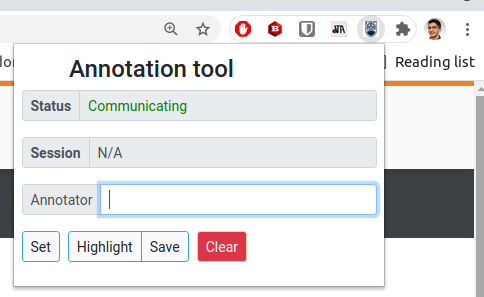
\includegraphics[width=\textwidth]{cp4/annotation-tool}
    \caption{Annotation tool and relevant sentences marked by an annotator}
    \label{fig:corpus-annotation-tool}
\end{figure}


Overall, annotation required a total of $\approx45$ hours of manual work \rev{divided across all the annotators}.
The annotation process was done throughout the course of 5 weeks.
% Appendix~\ref{apx:android-corpus} shows the instructions shared with the annotators.


% Annotation procedures for these tasks were analogous to the introductory tasks.










\subsubsection{Text inspected}





Annotators had to inspect a total of 12,401 sentences originating from API documentation, Stack Overflow answers, GitHub issue discussion and miscellaneous web pages.
These sentences comprise natural language written text---in this case, English---and do not involve source code snippets that may appear alongside the text.


Table~\ref{tbl:corpus-summary} gives insight into the number of sentences inspected per artifact type. 
We observe that API documents and miscellaneous web pages contain the highest number of sentences in our corpus.
This is not surprising because API documents often contain boilerplate text 
and all the information needed for the usage of an API element is usually found in a single document~\cite{robillard2011field}.
Miscellaneous web pages comprise blogs or tutorials, 
which often provide step-by-step instructions and accompanying examples, 
what likely explains the large number of sentences for this type of artifact~\cite{arya2020, Jiang2016b}.


The content of GitHub issues mostly resembles conversations~\cite{Rastkar2010}
and, beyond code snippets and minimal structured fields, the 
1,890 sentences inspected in this type of artifact comprise the description of a reported bug or a feature request as well as questions, answers, and discussion from  community members who are interested in resolving the issue at hand~\cite{zimmermann2010}.



For SO answers, the fewer number of inspected sentences (1,420) potentially relates to 
the fact that Stack Overflow offers little incentive for further discussion once a post has been answered.
Nonetheless, it is worthy noting that sentences with crucial information 
are not limited to the ones in an accepted answer~\cite{nadi2020}
and that later comments can be equally or more informative,
often providing notes about updates in an API component or framework~\cite{zhang2019so}.




\begin{table}[!h]
\centering    
\begin{small}
\begin{threeparttable}
\begin{tabular}{lccc}





& \multicolumn{3}{c}{\textbf{\# of sentences}}
\\ \cmidrule(l){2-4} 
& total & mean & stdv  \\

\hline
\hline

\textbf{API documentation} 
& 4,915 & 109.22 & 96.77
\\
\textbf{GitHub issues} 
& 1,890 &  43.95 & 33.69
\\
\textbf{SO answers} 
& 1,420 & 28.40 & 28.48 
\\
\textbf{Miscellaneous Web pages} 
& 4,176 & 70.78 & 56.64 
\\

\hline
\hline
\textbf{Overall} 
& 12,401 & 62.95 & 66.25 
\\
\hline

\end{tabular}
\end{threeparttable}
\end{small}
\caption{Summary statistics for the \acs{DS-android} corpus}
\label{tbl:corpus-summary}
\end{table}






\subsection{Corpus Description}
\label{cp4:corpus-description}


Overall, the resultant \acs{DS-android} corpus has
50 tasks and 133 artifacts, divided as 33 API documents, 45 Stack Overflow answers, 20 GitHub issues, and 35 other web pages.
Tasks in the dataset have an average of 3 associated artifacts each
and we discriminate the text marked by each annotator per artifact.
Overlap between the text marked by the annotators represents 30\% of the entire data 
and \textit{Krippendorff's alpha}~\cite{krippendorff2018} indicates 
 good reliability~\cite{Nenkova2004} over the text marked as relevant (or not) by the annotators ($\alpha=0.69$).



% \gm{Need to move table up so it is Table 4.3} -- OK
We structure tasks and annotation results in a format similar to the one shown in 
Table~\ref{tbl:corpus-data-structure}. 
Each task has a  title, link, description, and a set of pertinent artifacts.
In turn, each artifact has a type, title, link, and content,
where each sentence within an artifact's content
is preceded by the set of 
annotators (i.e., \texttt{none}, \texttt{A1}, \texttt{A2}, or \texttt{A3}) who marked the sentence as useful to the task.
As an example, in a Stack Overflow answer (artifact$_2$), all three annotators 
marked the sentence ``\textit{Have you checked RemoteControlClient?}''
as relevant to the lock mode task.



\afterpage{
    \begin{landscape}
\begin{table}
\begin{scriptsize}
% \vspace{-3mm}        
\begin{tabular}{cl}
\multicolumn{2}{l}{\cellcolor{lightgray}
    \textbf{Task}
}
\\
\multicolumn{2}{l}{\hspace{3mm}
\parbox[l][0.7cm][c]{16cm}{
    \texttt{No lock screen controls ever
}}}
\href{https://github.com/AntennaPod/AntennaPod/issues/3578}{link}
\\
\multicolumn{2}{l}{\cellcolor{lightgray}
    \textbf{Description}
}
\\
\multicolumn{2}{l}{
\hspace{3mm}
\parbox[l][2.5cm][c]{21cm}{
{\ttfamily
    \ldots
    \\
    \textbf{Expected behaviour:} Lock screen controls
    \\
    \textbf{Current behaviour:} No lock screen controls ever on this phone and never seen them working (or on preceding Huawei P8). Notification controls always work, never had problems. Lock screen controls fine for all other apps without tweaking, same on old P8. I have loosened all notification and lock screen limits, removed power management, etc., but no luck ever. I've also tried setting to use different players, but change in behaviour. \ldots
}}}
% --------------------------------------------------------------------------------------------------
\\
\hline
\hline
\multicolumn{2}{l}{\cellcolor{lightgray}
    \textbf{Artifact}$_1$ - \textbf{API documentation}}
\\
\multicolumn{2}{l}{\hspace{3mm}
\parbox[l][0.7cm][c]{16cm}{
    \texttt{Lock task mode Android Developers
}}}
\href{https://developer.android.com/work/dpc/dedicated-devices/lock-task-mode}{link}
\\
\multicolumn{2}{l}{\cellcolor{lightgray}
    \textbf{Content}}
\\
\texttt{none} & 
\parbox[l][0.6cm][c]{20cm}{
{\ttfamily    
    Android can run tasks in an immersive, kiosk-like fashion called lock task mode.
}}
\\
\texttt{A1} & 
\parbox[l][0.6cm][c]{20cm}{
{\ttfamily    
    Only apps that have been allowlisted by a device policy controller (DPC) can run when the system is in lock task mode.
}} 
\\
\texttt{none} & 
\parbox[l][0.6cm][c]{20cm}{
{\ttfamily    
    A DPC must allowlist apps before they can be used in lock task mode. 
}} 
\\
\texttt{A1, A2} & 
\parbox[l][0.6cm][c]{20cm}{
{\ttfamily    
    Call DevicePolicyManager.setLockTaskPackages() to allowlist apps for lock task mode as shown in the following sample
}} 
\\
\multicolumn{2}{c}{\texttt{...}}
% --------------------------------------------------------------------------------------------------
\\
\hline
\hline
\multicolumn{2}{l}{\cellcolor{lightgray}
    \textbf{Artifact}$_2$ - \textbf{Stack Overflow answer}}
\\
\multicolumn{2}{l}{\hspace{3mm}
\parbox[l][0.7cm][c]{16cm}{
    \texttt{Media Control on Lock Screen like Google Play Music in android?
}}}
\href{https://stackoverflow.com/questions/24652078/media-control-on-lock-screen-like-google-play-music-in-android}{link}
\\
\multicolumn{2}{l}{\cellcolor{lightgray}
    \textbf{Content}}
\\
\texttt{A1, A2, A3} & 
\parbox[l][0.6cm][c]{20cm}{
{\ttfamily    
Have you checked RemoteControlClient? 
}}
\\
\texttt{A2, A3} & 
\parbox[l][0.6cm][c]{20cm}{
{\ttfamily    
    it is used for the Android Music Remote control even if the App is in Lock mode.
}} 
\\
\multicolumn{2}{c}{\texttt{...}}
\\
\hline

\end{tabular}
\end{scriptsize}
\caption{Example of how data is structured in the \acs{DS-android} corpus. Each task has a  title, link, description, and a set of pertinent artifacts. Each artifact has a title, link, and content. For each of the sentences in the content, we store the set of annotators (i.e., \texttt{none}, \texttt{A1}, \texttt{A2}, or \texttt{A3}) who marked the sentence as useful to the task \red{UPDATE after annotation finishes}}
\label{tbl:corpus-data-structure}
\end{table}

\end{landscape}

}





Table~\ref{tbl:corpus-annotation-summary} provides summary statistics for the text marked by 
the annotators over all the artifacts inspected as well as on an artifact type basis according to the text marked by any annotator.    
On average the text deemed useful to a software task in the artifacts inspected comprises 
8.93 sentences per artifact per annotator.
We observe that the highest number of sentences marked originate from miscellaneous artifacts
while the lowest come from GitHub issue discussions. 
The high number of sentences marked in the former might relate to the more didactic nature of web tutorials~\cite{arya2020, Jiang2017}.
For the latter, the content on GitHub may be too project-specific which might 
prevent a developer performing a task in a different context from benefiting from most of the content found in this type of artifact.
For example, discussions about whether a certain design is the most appropriate~\cite{Viviani2019} might not extend to other projects, but instructions on how to use an API element might.






\begin{table}[H]
\centering    
\caption{Summary statistics for the text deemed useful by annotators across the artifacts inspected in the \acs{DS-android} corpus}
\label{tbl:corpus-annotation-summary}
\begin{scriptsize}
\begin{threeparttable}
\begin{tabular}{lcccccc}





& \multicolumn{3}{c}{\textbf{\# of sentences marked}}
& \multicolumn{3}{c}{\textbf{\% of sentences marked by}}
\\ \cmidrule(l){2-4} \cmidrule(l){5-7} 
& total & mean & stdv 
& 1 annot. & 2 annot. & 3 annot. \\

\hline

\textbf{API documentation} 
& 327 & 9.62 & 7.88
& 76\% & 16\% & 7\%
\\
\textbf{GitHub issues} 
& 146 & 4.87 & 3.37
& 74\% & 20\% & 6\%
\\
\textbf{SO answers} 
& 330 & 7.33 & 5.08
& 57\% & 22\% & 21\%
\\
\textbf{Miscellaneous Web pages} 
& 590 & 12.55 & 9.88
& 75\% & 17\% & 8\%
\\

\hline
\textbf{Overall} 
& 1393 & 8.93 & 7.78
& 71\% & 19\% & 10\%
\\
\hline

\end{tabular}
\begin{tablenotes}
    \item[annot] annotator(s);
\end{tablenotes}
\end{threeparttable}
\end{scriptsize}
\end{table}





Table~\ref{tbl:corpus-annotation-summary} also reports the percentage of sentences marked by one, two or the three annotators who inspect the artifacts in the corpus.
Our rationale for providing this data is that individuals might use different criteria to
assess the usefulness of a sentence to a given task~\cite{Barry1994, Barry1998}.
Out of 1,393
unique marked
sentences, 
10\% were marked by all annotators,
19\% by two of them and the remainder---996 sentences---by a single annotator.
These ratios follow Nenkova and Passonneau's empirical findings on 
content selection~\cite{Nenkova2004}
and are a similar to the ratios in the \acs{DS-synthetic} corpus,
where sentences marked by a single annotator comprise the majority of the data.
Although we leave the in-depth analysis of how an individual's background plays a role in what they perceive as relevant for future studies,  evaluation metrics should outline how 
the differences between the text marked are taken into account when 
using the golden data provided in our corpus. % for evaluation purposes



Based on the text marked by the annotators,   
we also ask if the amount of information required to solve a task was similar in GitHub or Stack Overflow tasks.
Answering this question will allow us to know whether 
the corpus can be evenly used for evaluation purposes or 
whether we must distinguish tasks according to their origin.
To answer this question, Table~\ref{tbl:corpus-annotation-summary-by-task} shows the number of sentences marked by any annotator according to a task's origin.
We use a Wilcoxon-Mann-Whitney test~\cite{mannWhitneyU} to check if there are any differences between the
average number of sentences marked per type of artifact in GitHub and Stack Overflow task.
Results show there is no statistically significant difference 
between the number of sentences  marked.
Hence, the corpus can be used for evaluation purposes without the need to distinguish tasks based on their origin.





\begin{table}[H]
\centering    
\caption{Number of sentences marked per type of task}
\label{tbl:corpus-annotation-summary-by-task}
\begin{scriptsize}
\begin{threeparttable}
\begin{tabular}{lcccccc}



& \multicolumn{3}{c}{\textbf{GitHub}} & \multicolumn{3}{c}{\textbf{Stack Overflow}} \\

& \multicolumn{3}{c}{\textbf{\# of sentences marked}} 
& \multicolumn{3}{c}{\textbf{\# of sentences marked}}
\\ \cmidrule(l){2-4}  \cmidrule(l){5-7} 

% Git
& total & mean & stdv 
%
& total & mean & stdv
\\

\hline

\textbf{API documentation} 
& 4,915 & 109.22 & 96.77 % Git
& 4,915 & 109.22 & 96.77 % SO
\\
\textbf{GitHub issues} 
& 4,915 & 109.22 & 96.77 % Git
& 4,915 & 109.22 & 96.77 % SO
\\
\textbf{SO answers} 
& 4,915 & 109.22 & 96.77 % Git
& 4,915 & 109.22 & 96.77 % SO
\\
\textbf{Miscellaneous} 
& 4,915 & 109.22 & 96.77 % Git
& 4,915 & 109.22 & 96.77 % SO
\\

\hline
\textbf{Overall} 
& 4,915 & 109.22 & 96.77 % Git
& 4,915 & 109.22 & 96.77 % SO
\\
\hline

\end{tabular}
\end{threeparttable}
\end{scriptsize}
\end{table}









% We provide further details on the annotators' background and the text marked by each individual in Table~\ref{tbl:corpus-summary-per-annotator}. 
% An average of 645 sentences were marked by the annotators (std 160.53) and 
% we also observe differences in the text marked.
% For example,
% the most experienced annotator---with 5 years of professional programming experience---had the
% least amount of text marked while less experienced ones leaned towards selecting more sentences.
% Although we leave the in-depth analysis of how an individual's background plays a role in what they perceive as relevant for future studies, the differences observed
% suggest that no unique set of task-relevant text exists~\cite{Nenkova2004}.
% Therefore, evaluation metrics should outline how these nuances are taken into account when 
% using the golden data provided in our corpus.


% % 






